% !TeX encoding=utf8
% !TeX spellcheck = en-US

\chapter{Classes}

\begin{figure}[h]
	\centering
	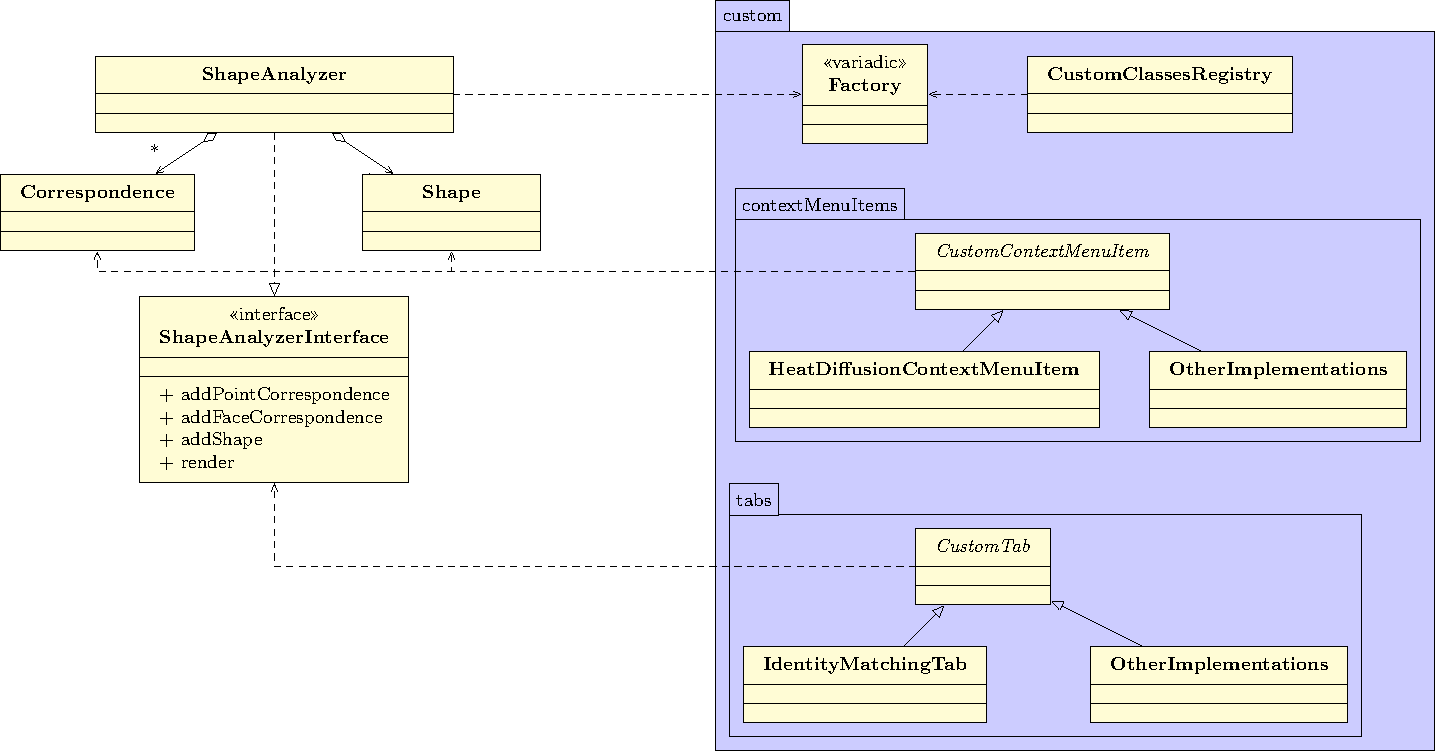
\includegraphics[width=\textwidth]{images/diagram.pdf}
\end{figure}

\begin{figure}[h]
	\centering
	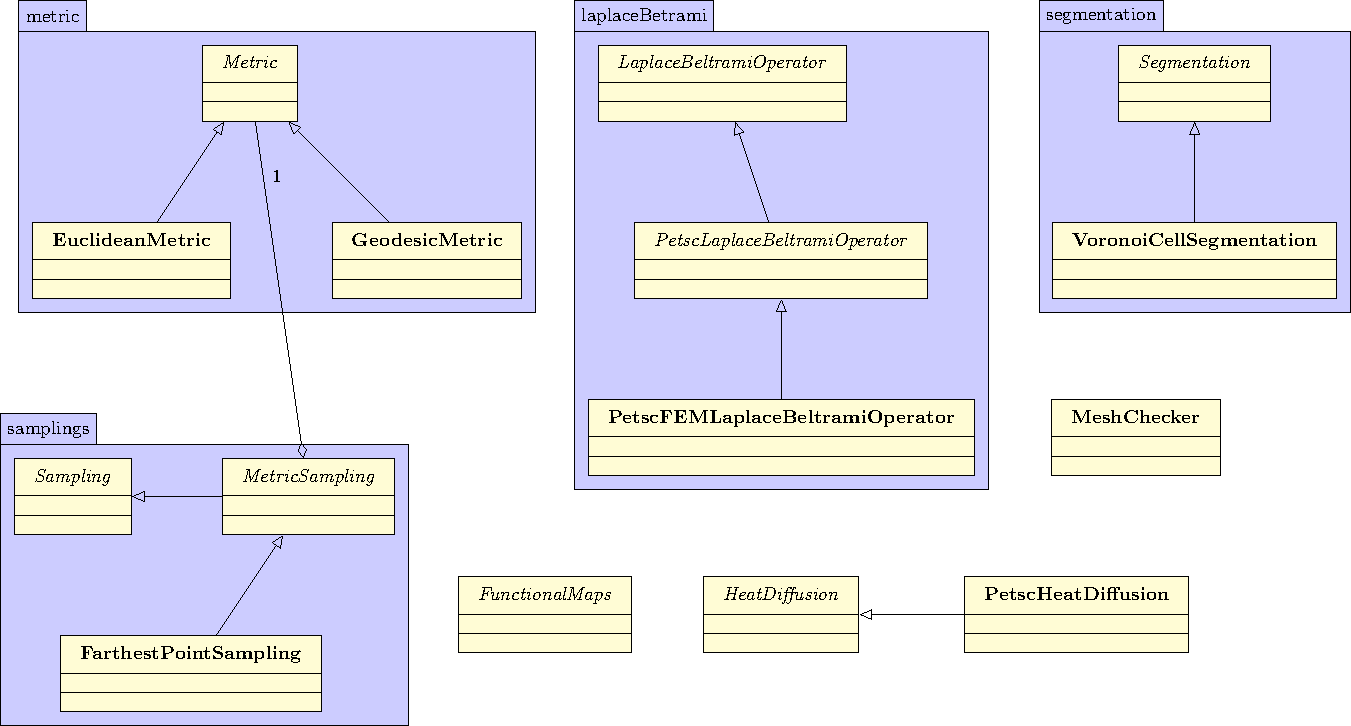
\includegraphics[width=\textwidth]{images/diagram2.pdf}
\end{figure}

\section{ShapeAnalyzer}
\label{sec:ShapeAnalyzer}

Blub.

\subsection{ShapeAnalyzerInterface}
\label{subsec:ShapeAnalyzerInterface}

\section{Shape}
\label{sec:Shape}

\section{Correspondence}
\label{sec:Correspondence}

\section{Factory}
\label{sec:Factory}

The Factory is responsible for automatically creating objects of Custom classes (see chapter \ref{chap:Customs}) and making them visible in the GUI. It is a variadic template that allows to specify the number and type of input parameters the constructors of those objects will get. It is realizing the Factory (you might have guessed it from the name) and the Singleton design pattern. 

\begin{mdframed}
If you only want your menu item / tab to appear in the GUI, no deeper knowledge of the Factory is required. Take a look at chapter \ref{sec:RegisterCustoms}. 
\end{mdframed}

\begin{lstlisting}[style=lstStyleCpp, caption={Factory.h}]
template<class T, class... Args>
class Factory {
    ...
    /// \brief Returns the unique instance of Factory<T>.
    /// \details This is the only way to obtain the Factory object for type T.
    static Factory<T, Args...>* getInstance() {
        static Factory<T, Args...> instance;
        return &instance;
    }
    ...
};
\end{lstlisting}

Due to the Singleton pattern there is only one Factory instance of every type. You can retrieve it by calling Factory<T, Args...>::getInstance() with the right template parameters. For example for CustomContextMenuItems there exist this Factory: 

\begin{lstlisting}[style=lstStyleCpp, numbers=none]
typedef Factory<CustomContextMenuItem, shared_ptr<Shape>, ShapeAnalyzerInterface*> CustomContextMenuItemFactory;
\end{lstlisting}

This Factory can produce CustomContextMenuItem objects that get a Shape and a ShapeAnalyzerInterface pointer as input parameters. As CustomContextMenuItem is an abstract class, the concrete classes have to be registered with a string identifier and a label. The string identifier has to be unique among all registered classes, the label will be shown in the GUI. 

\begin{lstlisting}[style=lstStyleCpp, caption=Factory.h]
template<class C>
    void Register(const string& identifier, const string& label) {
        // inserts a pair consisting of the identifier and a c++11 lambda 
        // expression calling the constructor of class C into the map 	
        // constructors
        function<T*(Args...)> constructor([](Args... args)->T* 
        		{ return new C(args...); });
        contructors_.insert(pair<string, function<T*(Args...)
        		>>(identifier, constructor));
        
        labels_.push_back(pair<string, string>(identifier, label));
        labelIndex_.insert(pair<string, int>(identifier, labels_.size() - 1));
}

T* create(const string& identifier, Args... args) {
        // execute create function pointer given the arguments in tuple args.
        return contructors_.at(identifier)(args...);
    }
\end{lstlisting}

The register function is a template taking the concrete class  as the template parameter \texttt{C}. It will create and store a lambda expression that calls the constructor of \texttt{C} with input parameters that were given as template parameters to the Factory template. Afterwards the create function will take the identifier and input parameters and use the stored constructors to create new objects. As the identifiers are stored separately, they can be used to automatically create objects of all registered classes. This happens when the menu is called.

\begin{lstlisting}[style=lstStyleCpp, numbers=none]
CustomContextMenuItemFactory::getInstance()>
Register<VoronoiCellsContextMenuItem<GeodesicMetric>>
("voronoicells_geodesic", "Segmentation>>Voronoi Cells>>Geodesic");
\end{lstlisting}

The label parameter allows to create layered menus. For menu items the label will be separated at every \texttt{>>}, creating a new sub menu. Menu items that have the same label up to some level will be put in the same sub menu. For tabs the label has to start with \texttt{"Shapes>>"} or \texttt{"Correspondences>>"} and no further sub menus will be created. 


